\documentclass{article}


\usepackage{arxiv}
\usepackage{amsmath}
\usepackage[utf8]{inputenc} % allow utf-8 input
\usepackage[T1]{fontenc}    % use 8-bit T1 fonts
\usepackage{xr-hyper}       % cross-references to the separate supplement
\usepackage{hyperref}       % hyperlinks
\usepackage{url}            % simple URL typesetting
\usepackage{booktabs}       % professional-quality tables
\usepackage{amsfonts}       % blackboard math symbols
\usepackage{nicefrac}       % compact symbols for 1/2, etc.
\usepackage{microtype}      % microtypography
\usepackage{lipsum}
\usepackage{graphicx}
\usepackage{amssymb}
\usepackage{natbib}

\graphicspath{ {./images/} }
\externaldocument{sup}


\title{Sparsity-driven emergence of functional modularity in multitask neural networks}


\author{Bowen Shi$^{1,2}$ \quad Qi Ouyang$^{1,3,4}$ \quad Long Qian$^{2,3}$\\
\small $^1$Institute for Advanced Study in Physics, Zhejiang University, Hangzhou 310058, China\\
\small $^2$Center for Quantitative Biology, Academy for Advanced Interdisciplinary Studies,\\
\small Peking University, Beijing 100871, China\\
\small $^3$ZJU--Hangzhou Global Scientific and Technological Innovation Center, Hangzhou 311200, China\\
\small $^4$Institute of Fundamental and Transdisciplinary Research, Zhejiang University, Hangzhou, China\\
\texttt{sbw1996@zju.edu.cn; qoy@zju.edu.cn; longqian@pku.edu.cn}
}


\begin{document}

\maketitle

\begin{abstract}

Neural networks can learn multiple tasks, but how learning organizes shared computation into specialized and reusable components remains poorly understood. In this work, we show that sparsity-inducing regularization promotes functional modularity in multitask networks without predefined module boundaries. Using functional profiling in multilayer perceptrons and a lightweight transformer, we identified compact, task-selective subnetworks, termed functional tokens. Across rule-based task families, selectively retaining these tokens preserves their associated functions while reducing performance on other tasks. Such specialization develops preferentially in deeper layers during training, while earlier layers retain shared computation. Regularization strength and form shape module compactness and specialization, while task weighting alters functional allocation. Moreover, extracted functional tokens can be recombined through alternative pathways to reconstruct a learned composite computation without retraining, preserving their connectivity and learned weights. Our results suggest that sparsity-constrained optimization shapes not only parameter use but also the organization and reuse of learned computation.

\end{abstract}

\section*{Significance statement (101, for PNAS)}
Understanding neural networks requires explaining not only their performance but also how their learned functions are organized. We show that encouraging a network to use fewer connections while learning multiple tasks promotes a division of labor without predefined module boundaries. Compact components specialize for different tasks while coexisting with shared computation. These components preserve their associated functions and can be reconnected to reconstruct a learned composite function without further training or changes to their learned weights. Our findings suggest that sparsity-constrained optimization can promote functional organization, and provide an experimental framework for studying how specialized and reusable computations emerge through learning.

\section{Introduction}

Deep neural networks have achieved wide success across perception, language, reasoning, and scientific discovery \cite{Bengio+chapter2007,Hinton06,goodfellow2016deep}. Despite substantial advances in architectural design \cite{heDeepResidualLearning2015,huangDenselyConnectedConvolutional2018} and optimization \cite{ruderOverviewGradientDescent2017}, the organizational principles that emerge during learning remain poorly understood. In particular, it is unclear how networks with distributed parameters and representations develop specialized functions while sharing and reusing computation across tasks. Biological intelligence provides a compelling example of such organization: functional modularity, characterized by partially independent yet interacting computational components, enables neural systems to support specialized processing, robustness, and compositional reuse across tasks \cite{damicelliTopologicalReinforcementPrinciple2019,margalitUnifyingFrameworkFunctional2024}.

Motivated by the computational advantages of modularity, previous machine-learning approaches have attempted to incorporate modular organization through explicit design. Neural module architectures introduce predefined functional components that can be selectively combined for different tasks \cite{andreasNeuralModuleNetworks2017,braylanReuseNeuralModules2015}, while adaptive structural learning methods seek to optimize network architectures by modifying connectivity patterns \cite{cortesAdaNetAdaptiveStructural2017,liuStructureLearningDeep2018}. Other approaches have explored structure-preserving constraints to incorporate prior organization into neural networks \cite{celledoniStructurepreservingDeepLearning2021}. More recently, sparse expert architectures have enabled large-scale neural networks to achieve conditional computation by routing inputs to specialized subnetworks \cite{shazeer2017outrageously,fedus2022switch}. Although these approaches demonstrate the utility of modular computation, they typically rely on architectural constraints, predefined components, or explicit routing strategies \cite{sunModularityDeepLearning2023}.

Modular organization, however, need not be specified in advance. Evolutionary studies have shown that modularly varying goals or selection to reduce connection costs can promote the emergence of modular networks \cite{kashtan2005spontaneous,clune2013evolutionary}. More recently, work on multitask recurrent networks has linked emergent modularity to task demands, representational capacity, and connection-growth dynamics \cite{wu2026taskstructured}. Learned modular connection masks can also improve subsequent learning after weight reinitialization, particularly under capacity constraints \cite{wu2026taskstructured}, demonstrating the utility of learned connectivity as a structural prior.

Sparsity provides an optimization-level route to investigate how constraints on connectivity shape computation. Sparsity-inducing regularization encourages a network to use fewer connections without prescribing internal module boundaries. Sparse and structured regularization have been extensively studied for model compression, parameter selection, and pruning \cite{wenLearningStructuredSparsity2016,scardapaneGroupSparseRegularization2017,maTransformed1Regularization2019}, while analyses of learned features, task-selective representations and shared dynamical motifs have revealed structure in trained networks \cite{agrawalWeightScaleInterpretingWeight2022,liGeometryConceptsSparse2024,michaudOpeningAIBlack2024,yangTaskRepresentationsNeural2019,driscollFlexibleMultitaskComputation2024}. The question here goes beyond network size: can sparsity help organize computation into task-selective components that preserve their associated functions and can be recombined with their learned parameters intact, without retraining?

In this work, we show that sparsity-inducing optimization can drive the emergence of functional modularity in multitask neural networks without explicitly designed modular architectures. Across multilayer perceptrons and a lightweight transformer, we identify compact, task-selective subnetworks, which we denote functional tokens, that coexist with shared computation. Across task families, these tokens preserve their associated functions under selective retention. By systematically varying sparsity strength and regularizer form, tracking functional specialization during training, and analyzing endpoint representation geometry, we characterize how sparsity shapes depth-dependent functional reorganization. Furthermore, extracted functional tokens can be connected through different pathways to reconstruct a learned composite computation without retraining or changing their learned parameter values. These findings connect sparse optimization to the organization and reuse of learned computation, highlighting machine-learning systems as models for uncovering general principles of computational organization \cite{levineMachineLearningMeets2024}.

\section{Results}

\subsection{Task-selective functional modules emerge under sparse multitask learning}

To examine how computation is shared and specialized across tasks, we used a controlled setting where a multilayer perceptron (MLP) with three fully connected ReLU hidden layers was trained to perform five related Binary Sequence Calculation tasks, without task-specific hidden branches or explicit modular routing (Fig.~\ref{fig:main1}a, Methods). The task set comprised four primitive arithmetic transformations, \(a + b\), \(ab\), \(a^{2}\), and \(b^{2}\), and one composite transformation \(a(a + b)\). Each shared input pair carried targets for all five rules, whose predictions occupied separate output blocks. The network was trained jointly on all rule losses from random initialization under sparsity-inducing \(L_{\gamma}\) regularization, with \(\gamma = 1\) as the default (Methods; Supplementary Note 5.1).

To map functional contributions across tasks, we individually silenced scalar weights and measured the resulting change in each rule's output segment (Fig.~\ref{fig:main1}b). Each scalar weight served as an elementary token. Rule-specific masks were constructed separately for each profiled weight matrix using the same extraction quantile, $\tau=0.75$; the numerical score thresholds were determined from each network, matrix and rule. Each selected weight was assigned an exact rule-set signature. A functional token for a rule or rule set retained the corresponding mask or union of masks simultaneously across all profiled weight matrices, including the output weights. Biases and other parameters outside the masking set remained unchanged (Methods; Supplementary Notes~\ref{appendix:Taylor} and~\ref{appendix:implementation}).

The resulting weight assignments revealed a depth-dependent organization (Fig.~\ref{fig:main1}c). Earlier hidden-layer weight blocks showed broader multi-rule support, whereas deeper blocks were enriched in sharper single-rule signatures and signatures involving fewer rules. This pattern was reproducible across independently trained networks.

We next examined whether retaining these supports preserved their associated computations. Rule-wise relative accuracy was defined as the retained subnetwork's accuracy divided by that of the corresponding full network on the same task. Single-rule functional tokens preserved substantial relative accuracy on their target rules, while performance on the other rules was reduced (Fig.~\ref{fig:main1}d). This selective preservation therefore provided a functional test of the extracted supports distinct from the individual-weight output perturbations used to define them. Multi-rule functional tokens likewise retained performance on their constituent tasks while remaining less effective on rules outside the selected rule set (Fig.~\ref{fig:main1}e,f). Exact rule-set signatures classify selected weights; subnetworks for a rule set retain the union of its rule-specific masks.



\begin{figure}[p]
    \centering
    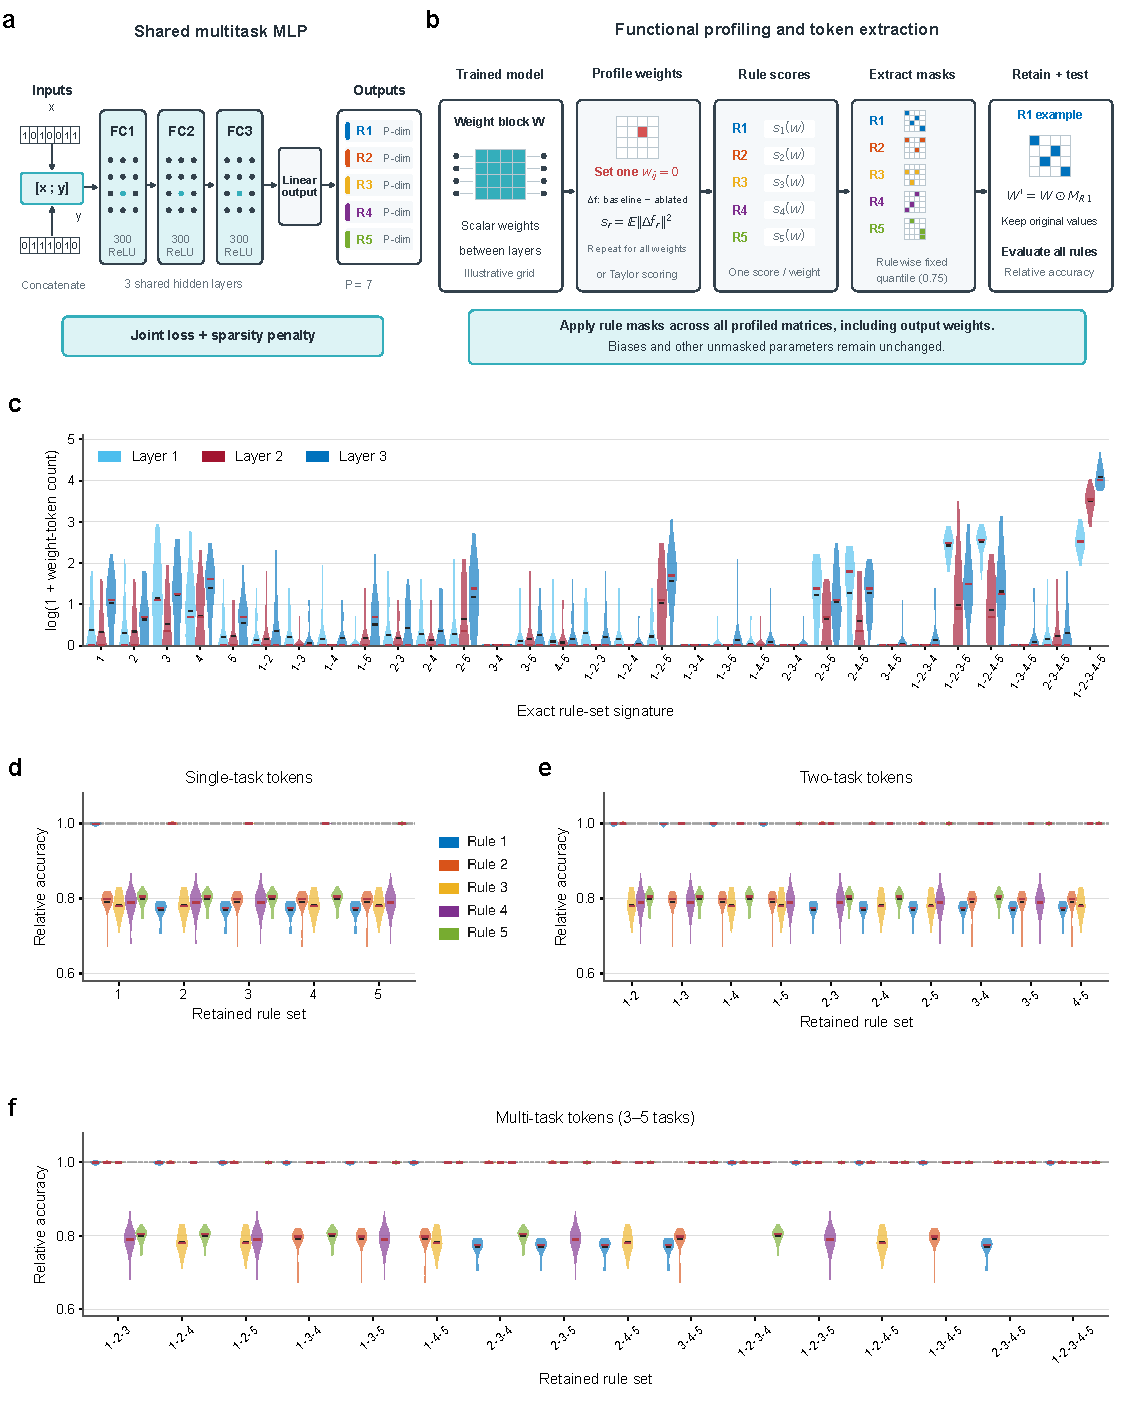
\includegraphics[width=\textwidth,height=0.81\textheight,keepaspectratio]{newfig/main_fig1.pdf}
    \caption{Network architecture, functional profiling and task-selective weight supports. (a) A shared MLP with three 300-unit ReLU hidden layers, trained jointly on five rules. (b) Functional profiling and extraction. Each scalar weight is scored individually by output ablation or Taylor output-sensitivity profiling. Rule-specific masks are constructed separately for each profiled weight matrix and then applied simultaneously across those matrices, including the output weights; biases and parameters outside the masking set are unchanged. (c) $\log(1+\mathrm{count})$ of weights assigned to each of the 31 nonempty exact rule-set signatures, shown separately for the three hidden-layer weight matrices. For example, ``1--3'' denotes the set $\{1,3\}$. (d--f) Relative accuracy of subnetworks retaining the union of masks for one rule (d), two rules (e), or three to five rules (f). Colours identify the evaluated rule. Relative accuracy is divided by that of the corresponding full network on the same rule. Violins summarize 30 independent runs; black and red marks indicate means and medians. Exact-signature counts in c and union-mask subnetworks in d--f are distinct summaries.}
\label{fig:main1}
\end{figure}



\subsection{Functional modularity persists across task families, profiling methods, and model architectures}

Having identified task-selective functional modules in the Binary Sequence Calculation setting, we next asked whether this organization depended on task semantics or input format, profiling criterion, or model architecture.

We first trained the same shared MLP architecture on two additional task families. Sparse Pattern Logic replaced arithmetic transformations with five Boolean-style rules, whereas MNIST Digit-Pair Arithmetic retained the arithmetic rule structure but presented pairs of digit images as inputs, coupling image-based input processing to arithmetic prediction (Methods; Supplementary Notes 5.2 and 5.3). Across independently trained networks for each task family, the extracted functional tokens preserved higher relative accuracy on their associated rules than on omitted rules (Fig.~\ref{fig:main3}a,b; Binary Sequence Calculation baseline in Fig.~\ref{fig:main1}d--f; Methods). Residual performance on omitted rules varied across task families, reflecting differences in computational overlap among the underlying transformations. Thus, the extracted subnetworks captured both task-selective and shared structure rather than imposing an artificial one-to-one partition between rules.



We next replaced exhaustive output ablation with randomized Taylor output-sensitivity profiling, a computationally less expensive criterion that estimates the squared first-order output perturbation associated with removing a scalar weight (Methods; Supplementary Note~\ref{appendix:Taylor}). The row-normalized mean relative-accuracy matrix for single-rule Taylor-derived tokens peaked on the corresponding evaluated rules (Fig.~\ref{fig:main3}c). This is a performance summary, not a matrix of Taylor gradients or importance scores.

Functional tokens extracted using the same score-quantile criterion retained high relative accuracy on their associated rules and showed reduced performance on other rules (Fig.~\ref{fig:main3}d). Thus, the two profiling criteria recovered consistent patterns of target-task sufficiency and off-task selectivity, indicating that the observed modular organization was not specific to a single importance measure. Similar performance patterns do not imply identical selected weight masks.

Finally, we trained a TinyTransformer on the same five-rule Binary Sequence Calculation task set (Fig.~\ref{fig:main3}e; Methods; Supplementary Note 2). Applying the Taylor-based profiling and retention procedure to scalar weight coordinates yielded functional tokens that preserved the corresponding target functions, with lower performance on omitted rules (Fig.~\ref{fig:main3}f). The extent of performance reductions varied across tasks. This architectural control extended the observation of task-selective functional organization beyond fully connected MLPs.



\begin{figure}[p]
\centering
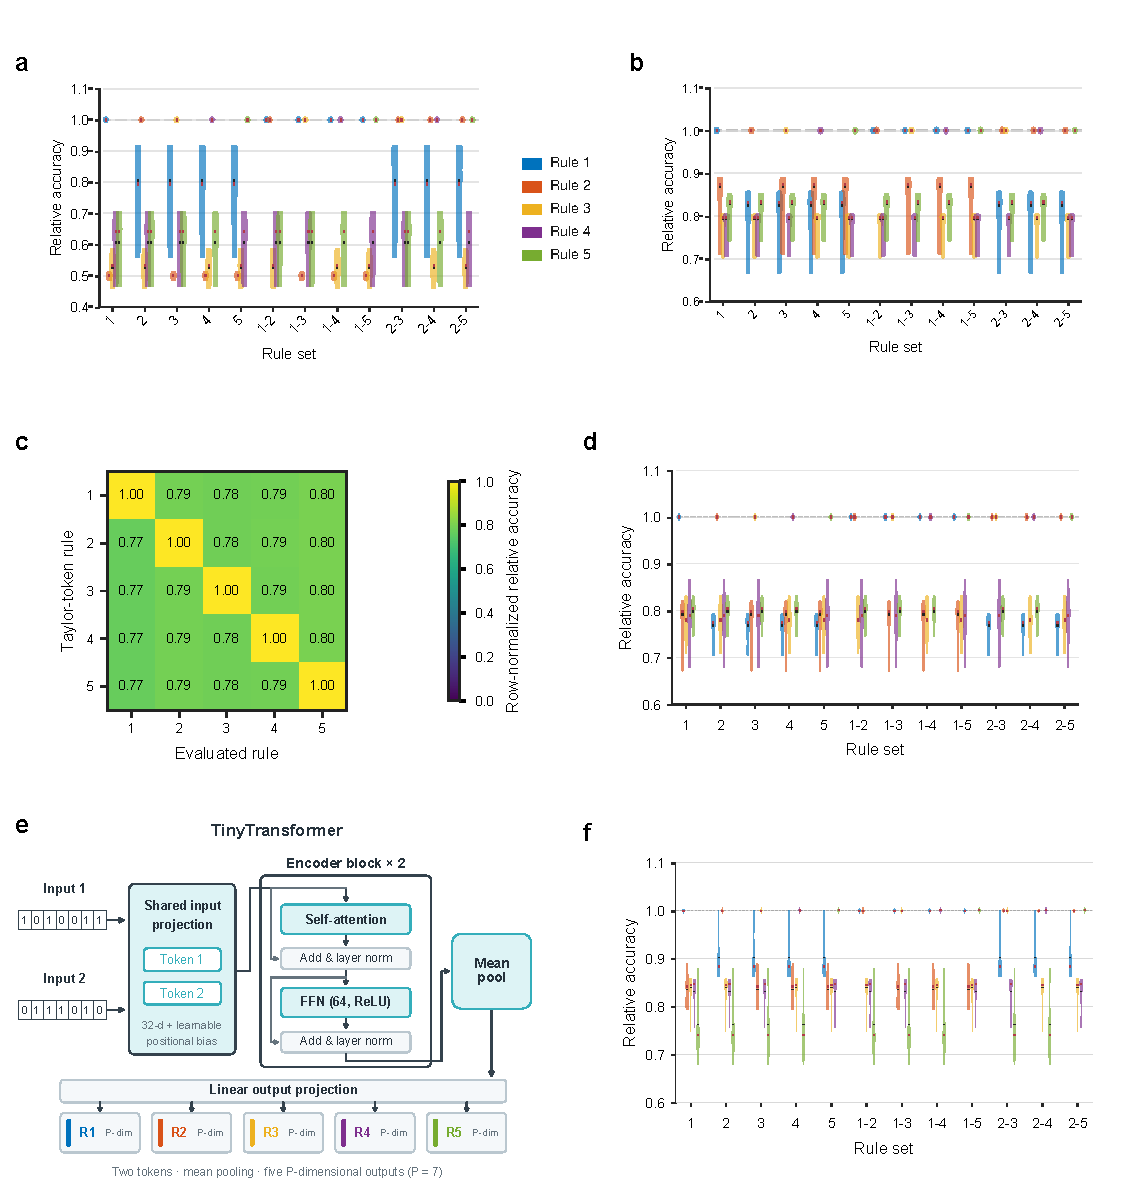
\includegraphics[width=\textwidth,height=0.82\textheight,keepaspectratio]{newfig/main_fig2.pdf}
\caption{Functional-token selectivity across task families, profiling methods and architectures. (a,b) Retained-mask relative accuracy for Sparse Pattern Logic and MNIST Digit-Pair Arithmetic, respectively. The Binary Sequence Calculation baseline is shown in Fig.~\ref{fig:main1}d--f. (c) Mean relative accuracy of single-rule Taylor-derived tokens, with each retained-token row normalized to its maximum; rows identify the retained-token rule and columns the evaluated rule. This is a performance summary, not a matrix of Taylor gradients or importance scores. (d) Relative accuracy of Taylor-derived MLP subnetworks. (e) TinyTransformer with two input tokens, a shared 32-dimensional projection and positional bias, two self-attention/FFN blocks with residual connections and layer normalization, mean pooling and a linear output head. (f) Taylor-derived TinyTransformer subnetworks in Binary Sequence Calculation. Violins summarize 30 independent runs in a,b,d and 23 batch-128 runs in f; black and red marks indicate means and medians. The scalar-weight masks are applied simultaneously to all profiled weight matrices, including the output projection; other parameters remain unchanged.}
\label{fig:main3}
\end{figure}

\subsection{Sparse regularization shapes the compactness and specialization of functional supports}

Having shown that task-selective functional organization persists across the tested settings, we next asked whether sparsity merely accompanies modularity or actively controls its emergence. Specifically, we interrogated the effects of the regularization strength $l$ and the regularization exponent $\gamma$ in the multitask MLP.

We first compared Lasso regularization strength \(l\) (\(\gamma = 1\)) with the non-regularized control (\(l = 0\)), re-extracting functional tokens from each trained network using the same ablation-based, within-rule score quantile criterion. For each \(l\) condition, three complementary quantities were assessed: target-rule relative accuracy, the retained scalar weight fraction, and the archived modularity statistic $M$ (Fig.~\ref{fig:main4}; Methods).

Without sparsity regularization, the extracted functional tokens retained comparatively large and diffuse supports and showed incomplete preservation of their target functions. Introducing \(L_{1}\) regularization at \(l = 1\) substantially improved target-rule relative accuracy while retained-weight fractions remained similar to those in the unregularized condition. Increasing the regularization strength to \(l = 5\) markedly reduced these fractions, with target-rule relative accuracy remaining close to the full-network level (Fig.~\ref{fig:main4}a). At $l=0$, the retained-weight ratio was close to one quarter, primarily reflecting the 75th-percentile extraction rule. It does not establish that one quarter of the full network is a naturally sufficient or minimal support. Ties at the threshold, finite-sample quantile interpolation and the additional score-floor filter can shift this ratio away from $0.25$.



The importance-weighted modularity distributions provided a complementary description of rule selectivity (Fig.~\ref{fig:main4}c,d). Increasing $l$ from 0 to 5 raised $M$ in the second and third hidden-layer weight blocks, followed by a plateau at $l=10$; the first block did not show the same monotonic response. These panels use ablation-derived, importance-weighted normalized inverse participation (NIP), as defined in Eq.~\eqref{eq:modularity}, with a fixed extraction quantile. The plotted distributions match the saved NIP results, and recomputation from representative trained checkpoints supports this identification (Methods; Supplementary Note~\ref{appendix:Taylor}). The observed plateau does not establish a universally optimal degree of sparsity.

We next asked whether these effects depended on the form of the regularizer. At fixed $l=5$, we compared ${L}_{\gamma }$ penalties with $\gamma \in \left\{0.5,1,2\right\}$ (Methods; Supplementary Note 2). The ${L}_{0.5}$ and ${L}_{1}$ penalties produced compact functional tokens that preserved target-rule performance and showed stronger deeper-block specialization, whereas the ${L}_{2}$ penalty yielded substantially larger retained-weight fractions, lower target-rule relative accuracy, and lower $M$ in deeper blocks (Fig.~\ref{fig:main4}b,d).

A local support-recovery analysis provides a conditional framework for interpreting both the dependence on regularizer form and the layer-specific response (Supplementary Note 1). Approximating hidden-layer computation or parameter-Jacobian effects by a multitask linear surrogate, the analysis identifies conditions on signal strength, feature coherence, and local approximation error under which sparse task supports can be recovered or locally stabilized. For $\gamma =1$, support recovery follows from a Lasso primal-dual witness argument; for $0<\gamma <1$, the nonconvex objective can admit an oracle-supported strict local minimum. In contrast, penalties with $\gamma >1$ primarily shrink weight magnitudes without enforcing exact sparsity \cite{zhaoModelSelectionConsistency,maTransformed1Regularization2019}. This distinction offers an interpretation of the contrast in Fig.~\ref{fig:main4}b,d: sparsity-inducing penalties can stabilize sparse task supports once compatible local coordinates emerge, rather than merely reduce weight magnitudes.

Theoretical analyses further indicate that support recovery or stabilization for \(0 < \gamma \leq 1\) depends critically on the coherence structure of the effective design, particularly the off-diagonal structure of the feature covariance. When active and inactive coordinates are sufficiently distinguishable, sparse regularization can more effectively eliminate redundant coefficients; strongly correlated features make exact support separation less stable. This dependence offers a possible interpretation of the observed depth profile. Early layer weights operate on common inputs and may retain intermediate features shared across tasks. Successive nonlinear transformations can produce coordinates in which task-relevant effects are more readily separated, allowing sparse penalties to concentrate rule-selective influence in later blocks closer to the rule-conditioned outputs while preserving shared computation near the input.



Together, retained-weight fraction, relative accuracy, and \(M\) distinguish support compactness, functional preservation, and specialization. The strength and form of sparse regularization shape how task-relevant influence is concentrated into compact, task-selective supports, while allowing shared computation to persist in earlier layer transformations.

\begin{figure}[p]
\centering
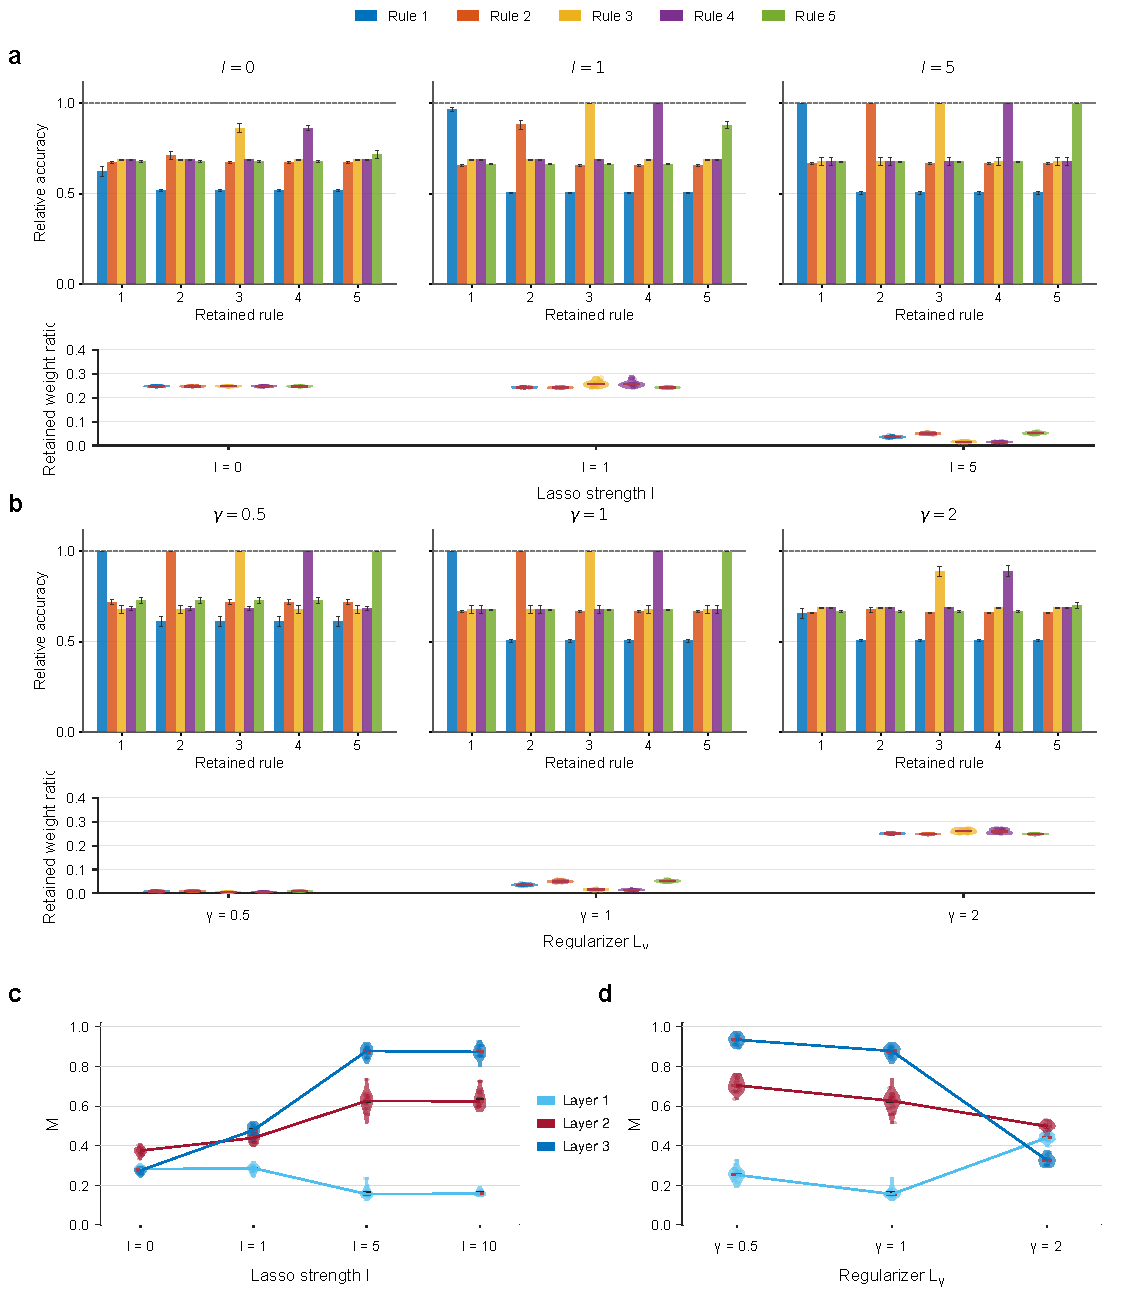
\includegraphics[width=\textwidth,height=0.81\textheight,keepaspectratio]{newfig/main_fig3.pdf}
\caption{Regularization changes the compactness and selectivity of extracted weight supports. (a) Relative accuracy on each evaluated rule for single-rule subnetworks at $l=0,1,5$ (upper plots), and retained-weight ratios (lower plot). (b) The corresponding quantities for $\gamma=0.5,1,2$ at $l=5$. Bars show means and error bars show sample SD across 30 independent runs. The retained-weight ratio is the number of mask-selected scalar coordinates divided by the total number of scalar coordinates in the analyzed weight matrices. It is not the nonzero-weight fraction of the full trained network. The extraction quantile is fixed at $\tau=0.75$; score thresholds are determined separately for each network, matrix and rule. (c,d) Layer-wise modularity across Lasso strengths (c) and regularizer exponents (d). Coloured guide lines connect medians for each layer at aligned x positions; these lines do not represent fitted functions. All panels use ablation profiling. Panels c,d show importance-weighted normalized inverse participation (NIP), defined in Eq.~\eqref{eq:modularity}. The adopted reproduction configuration uses $\epsilon_S=10^{-9}$, $\epsilon_{\mathrm{out}}=10^{-24}$ and all scalar-weight candidates (Methods).}
\label{fig:main4}
\end{figure}

\subsection{Depth-dependent functional specialization develops during training}

To determine how task-selective functional influence developed during optimization, we tracked the importance-weighted modularity score \(M\) at five saved checkpoints spanning 1,000--5,000 training epochs under Lasso strengths \(l \in \{ 0,1,5,10\}\) (Fig.~\ref{fig:main5}a). At each snapshot, scalar weights were Taylor-profiled and masks were recomputed within each hidden-layer weight block using the same rule-wise score-quantile criterion (\(\tau = 0.75\)). Each condition comprised 30 independent runs.

The trajectories were strongly dependent on both depth and regularization strength. Without regularization, median $M$ increased only modestly and reached 0.278, 0.375, and 0.277 in the three blocks at epoch 5000. At $l=1$, specialization accumulated more clearly in the second and third blocks, whose final medians were 0.440 and 0.481. Stronger regularization produced a more pronounced increase in the deepest block: between epochs 1,000 and 5,000, median $M$ rose from 0.516 to 0.883 at $l=5$, and from 0.731 to 0.874 at $l=10$. In contrast, the second block attained intermediate values and approximately plateaued, whereas the first block remained comparatively weakly specialized. Thus, task-selective importance progressively concentrated in the deepest block rather than increasing uniformly across the network. This layer-dependent temporal separation mirrors the final depth-dependent organization: early transformations retained broader multi-rule influence, whereas the deepest weight block progressively consolidated task-selective importance.

To characterize the representations accompanying this organization, we analyzed the latest saved epoch with \(\gamma = 1\) (Fig.~\ref{fig:main5}b--e; Supplementary Note 6). Pairwise-correlation distributions were estimated at \(l \in \{ 0,1,5,10\}\) from four independent runs per condition, whereas PCA and centered kernel alignment (CKA) analyses used 30 runs per condition over the extended sweep \(l \in \{ 0,1,2,3,5,10,15\}\).

In contrast to a simple monotonic-demixing account, Pearson correlations between pre-activation unit responses changed in a layer-dependent, non-monotonic manner (Fig.~\ref{fig:main5}b). The clearest increase in correlations near zero occurred in the first hidden layer at \(l = 1\). At stronger regularization, deeper layers instead redistributed more correlation mass toward intermediate values.



PCA spectral entropy revealed a complementary change in the distribution of representational variance (Fig.~\ref{fig:main5}c). Across the analyzed post-ReLU hidden and output representations, the pooled median entropy decreased from 3.279 at \(l = 0\) to 2.280 at \(l = 15\), indicating that representational variance became concentrated into fewer dominant directions. This indicates a redistribution of representational variance; it is distinct from the number of selected weight coordinates.

Linear CKA further showed that sparsity altered the division of representational roles across layers rather than simply reducing dimensionality uniformly (Fig.~\ref{fig:main5}d,e). Similarity among hidden-layer representations remained high across the sweep, peaked at moderate regularization, and declined modestly at larger $l$. By contrast, pooled hidden-output CKA increased from 0.418 at $l=0$ to 0.619 at $l=15$. Hidden representations therefore retained broadly compatible geometry while becoming progressively aligned with the rule-conditioned output space.

Together, the training trajectories show that sparse optimization preferentially strengthens task-selective influence in deeper weight blocks. Endpoint representation analyses associate this organization with concentrated variance and stronger hidden-output alignment, rather than uniform decorrelation across layers. These observations are compatible with the support-recovery interpretation (Supplementary Note 1), by which sparse task supports are most readily stabilized when active and inactive coordinates are sufficiently separable, which depends on the coherence of the effective design matrix as well as on signal strength and local approximation error. These activation-level correlations and representation similarities do not directly establish the effective-design coherence, signal-strength or score-margin assumptions required by the local support-recovery theory.

\begin{figure}[p]
\centering
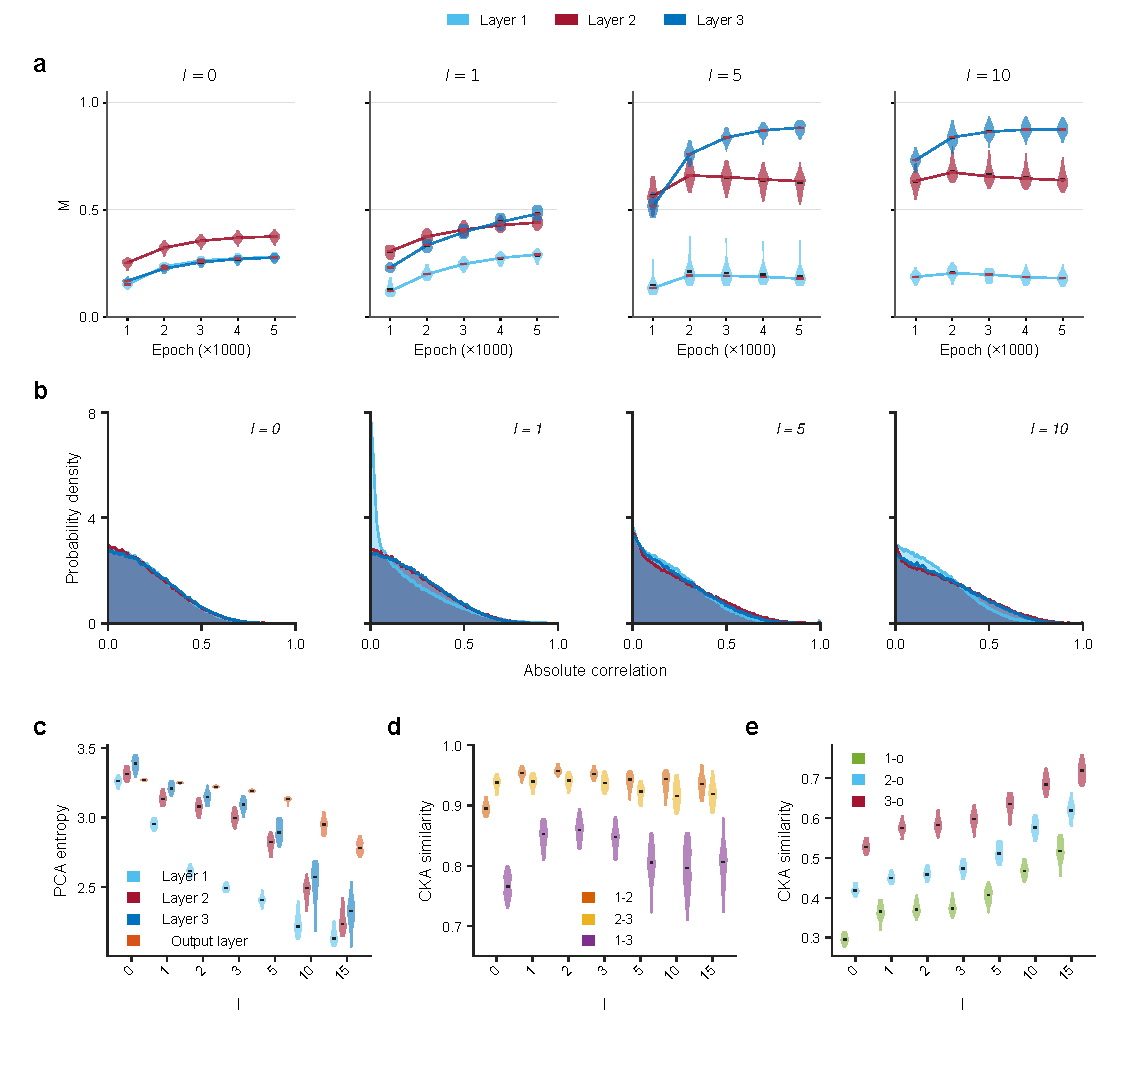
\includegraphics[width=\textwidth,height=0.82\textheight,keepaspectratio]{newfig/main_fig4.pdf}
\caption{Training dynamics and endpoint representation geometry. (a) Importance-weighted modularity $M$ at 1,000--5,000 epochs for $l=0,1,5,10$, from left to right, with $\gamma=1$. Violins show 30 independent runs; black and red marks show means and medians. Coloured guide lines connect medians within each layer at common epoch positions. Masks are recomputed at each snapshot using randomized Taylor output-sensitivity profiling with four probes and the same extraction quantile, $\tau=0.75$. The verified reproduction configuration uses $\epsilon_S=10^{-9}$, $\epsilon_{\mathrm{out}}=10^{-8}$, seed 0 and all scalar-weight candidates (Methods). (b) Distributions of absolute pre-activation unit correlations at the same four strengths, aligned column by column with a and pooled from four runs per condition. (c) PCA spectral entropy of post-ReLU hidden and output representations. (d) Hidden--hidden linear CKA. (e) Hidden--output linear CKA. Endpoint metrics in c--e use 30 runs per condition over $l=0,1,2,3,5,10,15$. Layer colours are consistent across panels; CKA legends identify the compared layer pairs.}
\label{fig:main5}
\end{figure}

\subsection{Task-biased optimization reshapes multitask performance and functional allocation}

Having examined how sparse regularization shapes functional organization, we next asked whether preferentially optimizing one task under sparse regularization improves its performance at the expense of other tasks, and how these changes relate to functional specialization. Without changing the network architecture or training data, we introduced per-rule weighting into the multitask objective:

\[\mathcal{L}=\frac{1}{R}\sum_r W_r\mathcal{L}_r+l_{\mathrm{train}}\Omega_\gamma(\theta).\]

where ${W}_{r}$ denotes the weight assigned to rule $r$. To emphasize a specific rule, we assigned ${W}_{r}=5$ while keeping unit weights for all other rules. All six conditions used three hidden layers of 300 units and were trained with $l_{\mathrm{train}}=5$ and $\gamma=1$, and each weighting condition was compared with an equal-weight control across 30 runs (Fig.~\ref{fig:main6}).

The full-network response depended on the emphasized rule (Fig.~\ref{fig:main6}a). Upweighting rules 2 or 5 improved mean accuracy not only on the target rule but also on all four non-upweighted rules. By contrast, emphasizing rules 3 or 4 improved target-rule accuracy while reducing mean accuracy on the other rules. Upweighting rule 1 reduced performance on both the target and non-target rules. Preferential task weighting therefore produced distinct outcomes, ranging from cross-task gains to target-specific gains accompanied by losses elsewhere.

To relate these performance changes to functional organization, we re-extracted functional tokens independently from each trained network using the same ablation-based score-quantile criterion. We quantified each token by its retained scalar weight fraction and its specialization margin, defined as its target-rule relative accuracy minus its mean relative accuracy on the other four rules (Supplementary Note 7). Support changes extended across rule-defined tokens: emphasizing rules 2 or 5 increased retained-weight fractions broadly, whereas emphasizing rule 1 reduced them. Rules 3 and 4 produced small increases in their own target-token supports, with mixed increases and decreases in non-target supports (Fig.~\ref{fig:main6}b). Thus, the observed performance trade-offs did not simply correspond to expansions of the target token accompanied by the contraction of the others.

Specialization margins further distinguished functional selectivity from preferential task performance. Conditions emphasizing rules 2 and 5 yielded margins of approximately 0.16--0.19 across the rule-defined tokens, whereas margins were substantially smaller under the rule-3 and rule-4 conditions that exhibited cross-task performance costs (Fig.~\ref{fig:main6}c).

Changes in target accuracy and retained-weight fraction were positively associated across the five target-rule means (Pearson \(r=0.73\); Fig.~\ref{fig:main6}d) and across 150 repeat-matched target-rule responses (\(r=0.78\), nominal \(p<10^{-4}\); Fig.~\ref{fig:main6}e). Target-performance gains therefore tended to accompany larger selected supports, but were not restricted to conditions with high functional selectivity. The pooled association comprises five upweighted-rule conditions with 30 repeat-matched responses per condition; it does not establish an independent effect after controlling for task identity and the shared control baseline (Supplementary Note~7).



\begin{figure}[p]
\centering
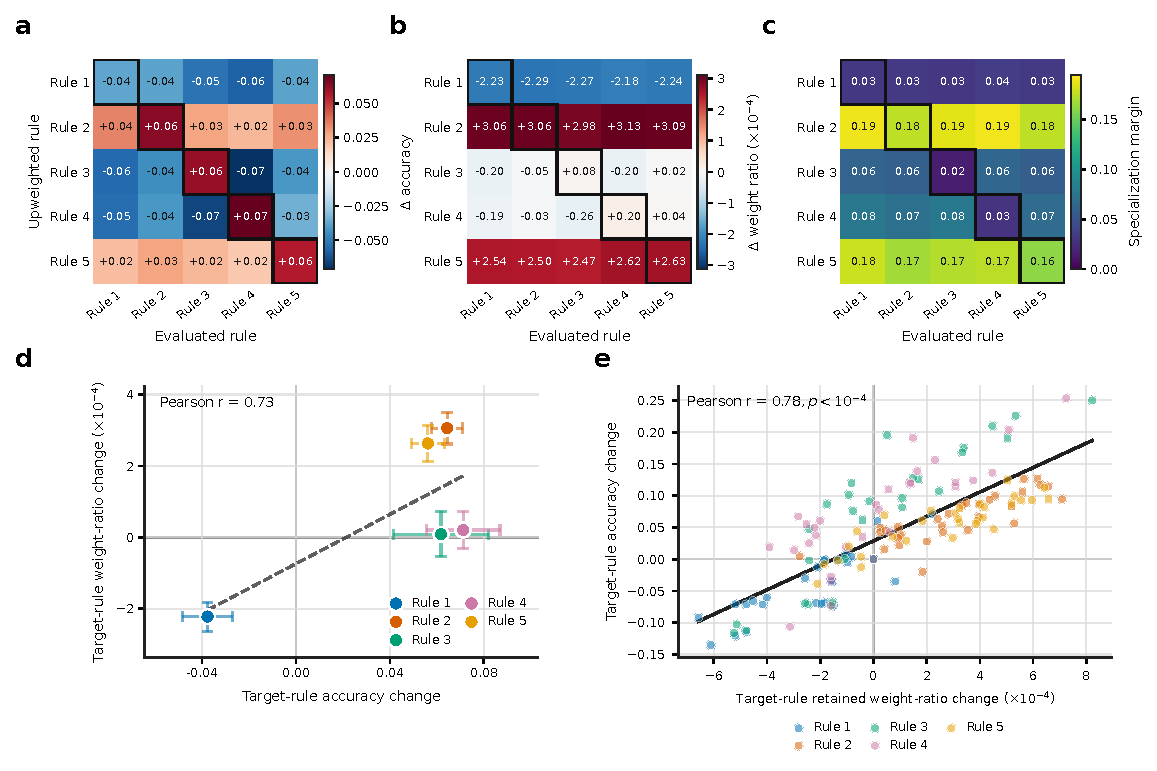
\includegraphics[width=\textwidth,height=0.71\textheight,keepaspectratio]{newfig/main_fig5.pdf}
\caption{Rule-loss weighting changes network performance and functional-token allocation. Five-rule MLPs were trained for 5,000 epochs with three 300-unit hidden layers, $l_{\mathrm{train}}=5$ and $\gamma=1$; one rule received five-fold loss weight, and each intervention was compared with an equal-weight control across 30 runs. (a) Change in full-network accuracy for each upweighted-rule and evaluated-rule pair. (b) Corresponding change in the retained scalar-weight fraction for each rule-defined functional token, displayed in units of $10^{-4}$. (c) Specialization margin: relative accuracy on the token's own rule minus its mean relative accuracy on the other four rules. Outlined diagonal cells in a--c identify the upweighted target. (d) Association between the five target-rule mean accuracy changes and retained-weight-ratio changes; error bars combine intervention and control marginal uncertainties as defined in Supplementary Note~7. (e) Association across 150 repeat-matched target-rule responses (30 repeats for each of five upweighted rules). Colours denote the upweighted rule; the line is a least-squares fit and the annotation reports the pooled Pearson correlation and nominal two-sided $p$ value, without adjustment for shared seeds and controls. These 150 points are not 150 independently sampled task identities.}
\label{fig:main6}
\end{figure}

\subsection{Learned functional tokens support compositional reuse without retraining}

Finally, we tested whether the extracted functional tokens could reuse their learned computations in explicitly specified composite pathways outside the configuration in which they were originally identified.

We considered the rule-5 Binary Sequence Calculation transformation,

\[f_5(a,b)=a(a+b)=a^2+ab.\]

which admits two equivalent decompositions through addition, multiplication, and squaring operations already learned by the same multitask network (Fig.~\ref{fig:main7}a). Because rule 5 was included in the mother network training, this experiment tested reconstruction of a learned composite function through alternative component connections.

For each Lasso strength \(l\), rule-specific functional tokens were extracted from a common mother network. Each component retained its extraction mask and learned parameters throughout recomposition: no component was retrained, fine-tuned, or merged with another mask (Supplementary Note 8). The directly extracted rule-5 token served as a non-recomposed control, with performance reported relative to the corresponding full mother network on rule 5.

In the type 1 pathway, the addition token first computed \(a + b\). Its thresholded output was paired with the original input \(a\) and passed to the multiplication token to implement \(a(a + b)\).

In the type 2 pathway, the square and multiplication tokens operated in parallel to compute \(a^{2}\) and \(ab\); their thresholded outputs were then passed to the addition token to implement \(a^{2} + ab\). Thus, the two pathways reconstructed the same target task through distinct computational graphs.

Both the sequential type 1 pathway and the parallel type 2 pathway recovered rule 5 with substantial relative accuracy (Fig.~\ref{fig:main7}b). Type 1 had a slightly higher mean than Type 2 at all four displayed regularization settings; at $l=5$ and $l=10$, both reached or slightly exceeded full mother-network performance. These results showed that rule-associated components could preserve useful computations after being connected through the specified intermediate interfaces.

Recomposition was also possible without regularization, but the associated functional supports were substantially larger and more diffuse. To relate reconstruction accuracy to support compactness, we defined the parameter-normalized reconstruction score \(E_{w}\):

\[E_w=\frac{A_{C,5}}{\rho_{\mathrm{nz},5}(l)}.\]

where $A_{C,5}$ is relative accuracy on rule 5 and $\rho_{\mathrm{nz},5}(l)=N_{\mathrm{nonzero},5}/N_{\mathrm{total}}$ is the nonzero scalar-weight fraction of the directly extracted rule-5 control (Supplementary Note~\ref{appendix:recomposition}). This differs from the mask-selected ratio $\rho_{\mathrm{mask}}$: a selected coordinate can have zero weight. The same denominator is used for the control and both recomposition pathways. $E_w$ increased with $l$ (Fig.~\ref{fig:main7}c), reflecting preserved reconstruction accuracy and a smaller reference support; it is not a pathway-specific parameter cost.

To assess the cost of obtaining functional tokens, we compared multitask training with and without token extraction against training five separate task-specific networks (Fig.~\ref{fig:main7}d; Supplementary Note~8.7). Across three auxiliary benchmark runs, the separate-training heuristic total was 4.78 times the joint-training-plus-extraction total. This comparison combines differently scaled training and extraction proxies; it is not a FLOP count, a measured speed-up, or a comparison at matched accuracy, and it excludes recomposition.



\begin{figure}[p]
\centering
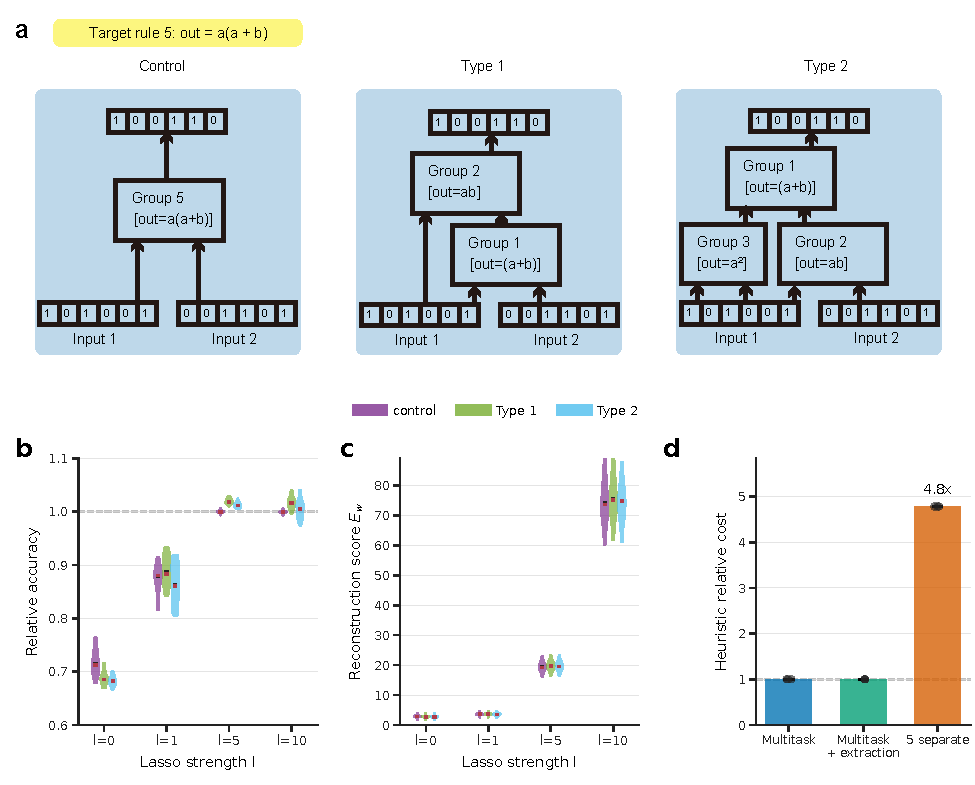
\includegraphics[width=\textwidth,height=0.71\textheight,keepaspectratio]{newfig/main_fig6.pdf}
\caption{Recomposition of learned functional tokens without retraining. (a) Recomposition of rule 5. The directly extracted rule-5 token is the control; Type 1 computes $a(a+b)$ sequentially, and Type 2 computes $a^2+ab$ through parallel primitives followed by addition. Component outputs are thresholded and encoded using the original task interface. Component masks and learned weights remain fixed. (b) Relative accuracy normalized to full mother-network rule-5 accuracy. (c) Parameter-normalized reconstruction score $E_w=A_{C,5}/\rho_{\mathrm{nz},5}(l)$, where $\rho_{\mathrm{nz},5}(l)$ is the nonzero scalar-weight fraction of the directly extracted rule-5 token, shared as the denominator across all three configurations. It is not the parameter count of each composite pathway. Violins summarize 30 independent runs per regularization setting, with means and medians in black and red. (d) Heuristic training/extraction cost comparison across three auxiliary benchmark runs: multitask training, multitask training plus extraction, and five separately trained networks. Bars show means, error bars s.e.m., and points individual runs. This proxy excludes recomposition and does not measure computational speed-up (Supplementary Note~8.7).}
\label{fig:main7}
\end{figure}

\clearpage
\section{Discussion}

Our results demonstrate that functional modularity can emerge under sparsity-constrained multitask learning, with compact, task-selective supports coexisting with shared computation. This organization recurs across the tested task families, profiling criteria, and architectures, while the MLP analyses reveal a systematic depth dependence. These findings complement work on explicit modular architectural design \cite{andreasNeuralModuleNetworks2017,sunModularityDeepLearning2023} and task-driven modular organization \cite{wu2026taskstructured} by identifying sparse optimization as a control of functional allocation and testing the preservation and reuse of learned computation.

Rather than treating parameter reduction as evidence of modularity, our analyses distinguish support compactness, functional preservation and specialization. Under the tested conditions, sparsity-inducing penalties produced smaller and more selectively organized supports than \(L_{2}\) regularization. Drawing on insights from Lasso consistency \cite{zhaoModelSelectionConsistency}, the local support-recovery analysis distinguishes sparse support formation from magnitude shrinkage and identifies conditions on signal strength, feature coherence, and approximation error under which recovery or local stabilization is possible (Supplementary Note~1). Its dependence on effective coordinates offers a possible interpretation of the depth profile: nonlinear transformations may make task-relevant effects more readily separable in later blocks, while early transformations retain shared computation. These activation-level correlations and representation similarities do not directly establish the effective-design coherence, signal-strength or score-margin assumptions required by the local support-recovery theory.

Training trajectories show that task-selective importance progressively concentrates in deeper blocks rather than increasing uniformly across the network. Separately, endpoint representation analyses associate this organization with concentrated variance and stronger hidden--output alignment, alongside layer-dependent, non-monotonic changes in neuronal correlations. These observations connect functional allocation to questions of feature geometry \cite{liGeometryConceptsSparse2024} and learned computational structure \cite{cagnettaTheoryHowStructure2024,chughtaiToyModelUniversality2023}, and resonate with neuroscientific accounts of modular specialization \cite{damicelliTopologicalReinforcementPrinciple2019}.

Task-biased optimization further distinguishes preferential task performance from functional specialization. Conditions with cross-task gains exhibited higher specialization margins than those with target--non-target performance trade-offs. Support changes also extended beyond the emphasized token rather than consistently following a target-expansion, non-target-contraction pattern. Cross-task costs therefore cannot simply be attributed to induced over-specialization. Instead, these results motivate evaluating functional selectivity jointly with performance across the task set, rather than treating greater task priority as a direct means of creating more isolated modules.

Methodologically, the functional-token framework connects importance profiling with tests of computational utility, complementing attribution-based interpretability approaches \cite{marcinkevicsInterpretableExplainableMachine2023,michaudOpeningAIBlack2024}. Retaining selected weights while simultaneously masking all profiled weight matrices, including output weights, preserved substantial target function and reduced off-target performance; biases and other unmasked parameters remained unchanged. Compositional reuse provides a further test: extracted functional tokens from a common mother network reconstruct a learned composite rule without retraining while preserving their masks and inherited weights. This evaluates reuse of learned computation, distinct from testing the learning performance of subnetworks trained in isolation under modular connection masks \cite{wu2026taskstructured}.

Taken together, these recomposition experiments demonstrate that identified functional tokens are neither static labels nor merely descriptive partitions of a trained network. Within the controlled task setting examined here, these properties support interpreting functional tokens as optimization-dependent and intervention-validated candidate sub-computations, while also showing that their reuse remains constrained by intermediate-interface compatibility and the selected computational decomposition.

Several limitations define the scope of this interpretation. Rule boundaries, primitive operations, composite relations, and task-specific readouts are specified by design, leaving open whether comparable supports can be recovered when tasks are implicit or component roles depend on context. Extraction depends on the intervention target, score normalization, and mask-selection criterion, and scalar-weight analyses may miss higher-order interactions or redundant pathways. The theoretical analysis should likewise be read as a local support-recovery argument for simplified linear surrogates. A stronger account would need to connect feature coherence, exact sparsity, representation geometry, and training-time dynamics in a single framework, and to specify when sparsity promotes separability versus when it destroys useful shared structure. Extending the framework to larger models should also test stability across extraction settings and datasets, compare weight-, path-, and circuit-level interventions, and evaluate targeted functional editing beyond masking.

\section{Methods}

\subsection{Model Architectures}

We conduct experiments using two representative neural architectures: a multilayer perceptron (MLP) and a lightweight transformer model (\textit{TinyTransformer}).

\subsubsection{Multitask MLP}

The multitask MLP consists of three fully connected hidden layers, each containing 300 ReLU units (Fig.~\ref{fig:main1}a). Each training sample comprises a shared input pair and labels for all selected tasks, and the output layer concatenates $R$ rule-specific predictions corresponding to $R$ distinct tasks. In the default setting, $R=5$, and the tasks consist of related arithmetic or logical transformations applied to the same input pair. All tasks are introduced simultaneously and optimized jointly from random initialization, without curriculum learning, sequential task presentation, or task-specific pretraining. Hidden activations are used for representation analyses, whereas functional-token extraction is performed on scalar weight coordinates in the trained parameter matrices. Sparsity is imposed using $L_\gamma$ regularization with $\gamma\in\{0.5,1,2\}$, with $\gamma=1$ used as the default unless otherwise stated. The task loss is averaged over the equally sized rule outputs, and the regularization penalty is the sum of the mean $(|w|+\varepsilon)^\gamma$ within each trainable non-bias weight matrix, with $\varepsilon=10^{-8}$. Additional architectural and training details, including the exact objective, are provided in Supplemental Information, Section~\ref{appendix:architecture}.

\subsubsection{TinyTransformer}

To test whether functional modularity generalizes beyond MLPs, we also consider a lightweight transformer encoder (Fig.~\ref{fig:main3}e). The model embeds the input into a compact sequence representation, applies a lightweight transformer encoder, and maps the pooled representation to the same multitask output format used by the MLP experiments. In the current experimental flow, the TinyTransformer control is trained on Binary Sequence Calculation rather than a token-tagging task. As in the MLP experiments, all tasks are trained jointly from random initialization, without curriculum learning or sequential task presentation. Functional-token extraction is performed on scalar weight coordinates. The TinyTransformer analysis includes 23 independent runs trained with batch size 128. Seven additional runs trained with batch size 500 are excluded to keep the training batch size uniform within this analysis; their original training records and analysis exports are retained. Full implementation details are provided in Supplemental Information, Section~\ref{appendix:architecture}.

\subsection{Task Design and Random Multitask Training}
\label{method:task_design}

We use several rule-based multitask families to test whether functional tokens emerge across different input formats and rule semantics (Supplemental Information, Section~\ref{appendix:tasks}). In all cases, a single shared neural network receives one input sample and predicts the concatenated outputs of the selected rules. Unless otherwise stated, experiments use the first five rules of the selected task family as the default multitask setting ($R=5$). Additional rules from the same family are used only when an experiment explicitly probes task-set expansion or alternative composite/identity controls.

For Binary Sequence Calculation tasks, each input consists of two binary vectors of length $P=7$. The complete task family contains six arithmetic rules. Rules~1--4 are independent primitive transformations--addition, multiplication, $a^2$, and $b^2$--whereas rules~5 and~6 are composite transformations, $a(a+b)$ and $b(a+b)$, which reuse primitive arithmetic structure. The default setting jointly trains rules~1--5, placing four primitive tasks and one composite task in the same shared network.

Sparse Pattern Logic tasks use the same paired binary-input format but replace arithmetic with elementwise logical operations. The full rule family contains AND, OR, XOR, NOT of the first input, identity of the first input, and identity of the second input; the default setting again uses the first five rules. MNIST Digit-Pair Arithmetic tasks mirror the Binary Sequence Calculation rule structure but use digit-derived inputs, testing whether the same extraction framework remains informative beyond direct synthetic binary variables. The TinyTransformer control uses the Binary Sequence Calculation setting with the same five default rules.

For each independent trial, examples are randomly sampled and split into training and validation sets. Labels for all selected rules are generated on the same samples, and all task losses are optimized jointly from random initialization. Thus, the model is trained in a randomized multitask setting, with all selected rules presented through shared mini-batches and without curriculum learning, sequential task presentation, task-specific pretraining, or hand-specified modular routing. Additional implementation details are provided in Supplemental Information, Section~\ref{appendix:architecture}.

\subsection{Profiling Functional Tokens}

\subsubsection{Ablation Profiling}
For each trained network and rule $r$, we quantify the functional contribution of a scalar weight token $q$ by zeroing that weight while keeping all other parameters fixed. Let $f_r(x)$ denote the baseline output block for rule $r$, and let $f_r^{(-q)}(x)$ denote the output after ablating scalar weight $q$. The ablation score is
\begin{equation}
S^{\mathrm{abl}}_{r,q}
=\mathbb{E}_{x\sim\mathcal{D}_r}
\left\|f_r(x)-f_r^{(-q)}(x)\right\|_2^2 .
\end{equation}
This score measures the output perturbation induced by removing one scalar weight coordinate from the trained model.

\subsubsection{Taylor Profiling}
As a complementary first-order approximation, we estimate the squared output sensitivity of each scalar weight:
\begin{equation}
S^{\mathrm{tay}}_{r,q}=\theta_q^2\,\mathbb{E}_x\left\|\frac{\partial f_r(x;\theta)}{\partial\theta_q}\right\|_2^2.
\label{eq:taylor_output}
\end{equation}
This approximates the squared first-order output perturbation associated with removing a scalar weight; it is not a task-loss gradient attribution. For each batch $B$, rule $r$ and probe $k=1,\ldots,K$, independent Rademacher signs $z_{i,d}^{B,k,r}\in\{-1,+1\}$ are drawn for each sample $i$ and output coordinate $d$. The estimator is
\begin{equation}
g_{B,k,r,q}=\frac{\partial}{\partial\theta_q}\sum_{i\in B}\sum_{d=1}^{P}z_{i,d}^{B,k,r}f_{r,d}(x_i;\theta),\qquad
\widehat S_{r,q}=\frac{1}{NK}\sum_B\sum_{k=1}^{K}(\theta_q g_{B,k,r,q})^2.
\label{eq:taylor_probe}
\end{equation}
Here $N$ is the total number of profiled samples. The expectation over the probes equals $\theta_q^2N^{-1}\sum_i\|\partial f_r(x_i)/\partial\theta_q\|_2^2$. There is no additional division by the output dimension $P$. The confirmed Taylor runs in Figs.~\ref{fig:main3}c,d,f and~\ref{fig:main5}a used $K=4$; this finite probe count does not itself guarantee a small uniform estimation error.

\subsection{Functional Token Extraction}

A weight token is a scalar coordinate in a trainable non-bias weight matrix. A rule-specific functional token is the set of weight tokens selected by an intervention-defined important mask. For each rule $r$ and weight token $q$, let $S_{r,q}\ge 0$ denote the corresponding importance score from ablation or Taylor profiling. To account for differences in output scale across rules, we also compute a normalized score profile
\begin{equation}
G_r=\mathbb{E}_{x\sim\mathcal{D}_r}\|f_r(x)\|_2^2+\epsilon_{\mathrm{out}},
\qquad
Q_{r,q}=\frac{S_{r,q}}{G_r},
\end{equation}
where $\epsilon_{\mathrm{out}}$ stabilizes output-energy normalization; it is distinct from the score floor $\epsilon_S$.

The extraction quantile is fixed at $\tau=0.75$. For each trained network $n$, profiled weight matrix $b$ and rule $r$, the numerical threshold is
\begin{equation}
T_{n,b,r}=\operatorname{Quantile}_{0.75}\{S_{n,b,r,q}:q\in\mathcal C_{n,b},\ S_{n,b,r,q}\text{ finite}\},
\end{equation}
where $\mathcal C_{n,b}$ is the set of profiled candidate coordinates. The important mask is
\begin{equation}
I_{n,b,r,q}=\mathbf{1}\{S_{n,b,r,q}\text{ finite}\}\mathbf{1}\{S_{n,b,r,q}>\epsilon_S\}\mathbf{1}\{S_{n,b,r,q}\ge T_{n,b,r}\}.
\label{eq:important_mask}
\end{equation}
The quantile is computed before score-floor filtering, so finite zero scores enter its calculation. The numerical threshold is recomputed for every network, matrix and rule, and at every profiled training snapshot. Fixed $\tau$ is not a fixed numerical score threshold. Legacy configuration fields \texttt{cutoff\_mode=fixed}, \texttt{panel\_a\_threshold} and \texttt{score\_ratio\_threshold} do not set the threshold in this \texttt{score\_quantile} branch. If a candidate cap is supplied, the implementation profiles at most that many coordinates per matrix, chosen by absolute weight magnitude; unprofiled coordinates are not selected. For a rule set $C$, masks are combined by union,
\begin{equation}
I_{C,b,q}=\max_{r\in C}I_{r,b,q}.
\end{equation}
We construct a mask separately for each profiled weight matrix and apply all masks simultaneously, including the output weights. Biases and other parameters outside the masking set remain unchanged. This subnetwork intervention differs from zeroing one scalar weight at a time to compute its importance. The retained-weight ratio is
\begin{equation}
\rho_{\mathrm{mask}}(C)=\frac{\sum_b\sum_{q\in W_b}I_{C,b,q}}{\sum_b|W_b|}.
\label{eq:retained_mask_ratio}
\end{equation}
Its numerator counts mask-selected positions, including selected coordinates with zero weight; its denominator counts all scalar coordinates in the analyzed weight matrices, including zero-valued entries and excluding biases. It is not the nonzero fraction of the full network.

We evaluate rule-wise \emph{relative accuracy} as
\begin{equation}
A(C,r) = \frac{A'(C,r)}{A_0(r)},
\label{eq:eq3}
\end{equation}
where $A'(C,r)$ is the accuracy of the retained subnetwork on rule $r$, and $A_0(r)$ is the accuracy of the full network on the same rule. This normalization reduces confounding from task difficulty when comparing robustness across task families. Unless otherwise stated, rule accuracy is the mean agreement over samples and output bits after binarizing predictions at $>0.5$, rather than the fraction of entirely correct output vectors. Relative accuracy uses this bitwise measure for both networks.

For descriptive assignment plots, a selected weight token can also be given an exact rule-set signature,
\begin{equation}
\sigma(q)=\{r:I_{r,q}=1\}.
\end{equation}
These signature counts visualize which rule combinations share selected weights; they are not used to define the modularity statistic.

The importance-weighted normalized inverse participation (NIP) statistic used in Fig.~\ref{fig:main4}c,d and the training trajectories in Fig.~\ref{fig:main5}a uses the masked score profile directly. Given a rule set $R$ and a block-specific important mask $I_{r,q}$, define
\begin{equation}
V_{r,q}=I_{r,q}\max(Q_{r,q},0),
\qquad a_q=\sum_{r\in R}V_{r,q}.
\end{equation}
Tokens are active when $a_q>\epsilon_M$, with $\epsilon_M=10^{-12}$, a numerical mass floor distinct from the raw-score floor $\epsilon_S$. For active tokens, let $p_{r,q}=V_{r,q}/a_q$. We define the normalized concentration
\begin{equation}
\phi_q=\sum_{r\in R}p_{r,q}^2,
\qquad
z_q=\frac{\phi_q-1/|R|}{1-1/|R|},
\end{equation}
and the block modularity score
\begin{equation}
M=\frac{\sum_{q:a_q>\epsilon_M}a_q z_q}{\sum_{q:a_q>\epsilon_M}a_q}.
\label{eq:modularity}
\end{equation}
Thus $M\in[0,1]$ measures the degree to which important weighted score profiles are concentrated on individual rules, with larger values indicating stronger functional specialization under a fixed extraction criterion. Masks are recomputed separately for each network, weight matrix, rule and snapshot. If no token is active, $M$ is undefined (returned as NaN).




\subsubsection{Configuration provenance}
The saved summaries for Figs.~\ref{fig:main1}c--f and~\ref{fig:main3}a,b,d,f record $\tau=0.75$, $\epsilon_S=10^{-9}$, $\epsilon_{\mathrm{out}}=10^{-8}$ and no candidate cap; the score floor is also present in all 150 original analysis exports. The current figures use 143 of these exports: 120 MLP exports and 23 TinyTransformer exports. Seven TinyTransformer runs trained with batch size 500 are excluded from Fig.~\ref{fig:main3}f, leaving the 23 runs trained with batch size 128; all original exports are preserved. The Taylor groups record four probes.

For reproducibility, we specify the current analysis configuration for Figs.~\ref{fig:main4} and~\ref{fig:main5}a: $\tau=0.75$, $\epsilon_S=10^{-9}$, all scalar-weight candidates, all available test samples and an analysis batch size of 64. Fig.~\ref{fig:main4} uses ablation profiling with $\epsilon_{\mathrm{out}}=10^{-24}$; Fig.~\ref{fig:main5}a uses randomized Taylor profiling with $\epsilon_{\mathrm{out}}=10^{-8}$, four probes and seed 0. The verified execution devices are CUDA for ablation and CPU for Taylor; fixing the Taylor device preserves the random-probe sequence. These settings define the adopted reproduction protocol.

The Fig.~\ref{fig:main4}c,d distributions match the saved importance-weighted NIP results and implement Eq.~\eqref{eq:modularity}; rule-count purity is a different statistic and was not used for these panels. Recomputing six representative ablation checkpoints with the adopted configuration gave a maximum absolute difference in $M$ of $1.04\times10^{-7}$, identical active-token counts, and identical single-rule relative accuracies and retained-weight ratios. Recomputing all 600 Taylor checkpoints underlying Fig.~\ref{fig:main5}a gave a maximum absolute difference in $M$ of $1.60\times10^{-8}$ and identical active-token counts. These checks reassess saved trained models rather than retrain them.

For Fig.~\ref{fig:main6}, all 180 newly trained 300-unit models underwent fresh scalar-weight ablation profiling. Fig.~\ref{fig:main7}b,c uses fresh profiling of all 120 saved 300-unit mother models, and Fig.~\ref{fig:main7}d and Supplementary Fig.~\ref{fig:training_cost} use fresh profiling of three saved auxiliary joint models. All these analyses use $\tau=0.75$, $\epsilon_S=10^{-9}$, $\epsilon_{\mathrm{out}}=10^{-8}$, perturbation batch size 64 and no candidate cap. All 194,700 scalar weights, including the output matrix, are candidates; masks are constructed separately per matrix and applied simultaneously, while biases remain unchanged. Fig.~\ref{fig:main6} uses $l_{\mathrm{train}}=5$ and $\gamma=1$, without display rescaling. The recomposition conditions retain the sweep's experiment/display strength mapping. The saved $10^{-6}$ score-ratio field is not a selection threshold in the \texttt{score\_quantile} branch, and probe-count metadata in ablation exports do not imply Taylor profiling.

Training regularization strength $l_{\mathrm{train}}$, extraction quantile $\tau$, realized score threshold $T$, score floor $\epsilon_S$ and output-energy constant $\epsilon_{\mathrm{out}}$ have distinct roles. In the saved Lasso/exponent sweep used for Figs.~\ref{fig:main4} and~\ref{fig:main5}, the displayed strength is $l=5l_{\mathrm{train}}$. Thus displayed $l=0,1,5,10$ corresponds to $l_{\mathrm{train}}=0,0.2,1,2$. This mapping is not assumed for experiments lacking corresponding historical records. Further per-experiment provenance is provided in Supplementary Note~\ref{appendix:Taylor}.

\subsubsection*{Supplemental Information}

Supplemental theoretical analysis, model and training details, task definitions, and supporting analyses are provided in the separate Supplemental Information document.

\subsubsection*{Data and Code Availability}

All synthetic datasets are generated by the task procedures described in Methods and Supplemental Information. MNIST-based experiments use the public MNIST dataset. Training, analysis, and figure-generation code are maintained in the accompanying project repository.

\subsubsection*{Acknowledgements}

This work was supported by the Beijing Natural Science Foundation (Z260005 to L. Q.) and the Fundamental and Interdisciplinary Disciplines Breakthrough Plan of the Ministry of Education of China (JYB2025XDXM502 to Q. O.).

\subsubsection*{Author contributions}

L. Q. and Q. O. conceived the study and designed the overall research framework. B. S. developed the theoretical methodology, designed and carried out the computational experiments and conducted data analysis. L. Q. supervised the research. B. S. and L. Q. wrote the manuscript with input from all authors. All authors discussed the results, reviewed the manuscript, and approved the final version.

\subsubsection*{Competing interests}

The authors declare no competing interests.

\bibliographystyle{unsrtnat}

\bibliography{ref}

\end{document}
